\documentclass[a4paper]{article}
\usepackage{subfiles}
\usepackage{amsmath, amssymb, amsthm}
\usepackage{mdframed}
\usepackage{tikz}
\usepackage{tikz-cd}
\usepackage{hyperref}

\usepackage{mdframed}

\newcommand*{\R}{\mathbb{R}}
\newcommand*{\C}{\mathbb{C}}
\newcommand*{\N}{\mathbb{N}}
\newcommand*{\Z}{\mathbb{Z}}
\newcommand*{\Q}{\mathbb{Q}}
\newcommand*{\F}{\mathbb{F}}
\newcommand*{\Pb}{\mathbb{P}}

\newtheorem{theorem}{Theorem}
\newtheorem{lemma}{Lemma}
\newtheorem{corollary}{Corollary}
\newtheorem{definition}{Definition}
\newtheorem{proposition}{Proposition}
\newtheorem{remark}{Remark}
\newtheorem{example}{Example}

\begin{document}
\author{Maxence Jauberty}
\title{An introduction to majorization and some personal thoughts about it}
\maketitle
\begin{abstract}
    The following article is \textit{somehow} an introduction to the theory of majorization.
    Its objective is to present the main ideas of the theory, as well as some personal thoughts about it.
    The reader can a complete introduction to the theory in \cite{marshall2011inequalities}.

    I would assume some basic knowledge in linear algebra, probability theory and familiarity with information theory.
\end{abstract}
\section{Introduction}
Majorization is a concept that appears in various fields of mathematics whenever we need 
to talk about \text{non-uniformity}, or \textit{randomness}.  
Many approaches are possible depending on the field, you are working on. A satisfying definition, giving
a general intuition of it, is given using the concept of Lorenz curve.
\begin{definition}[Lorenz Curve] Let \(x\in\Delta_n\), the Lorenz curve \(\mathcal{L}_x\) of \(x\) is the plot of the points 
\(\biggl(\frac{i}{n}, \sum_{j=1}^i x_{(j)}\biggr)\), where \(x_{(1)}\geq x_{(2)}\geq \ldots \geq x_{(n)}\) are the components of \(x\) in decreasing order.
\end{definition}
\begin{figure}
    \centering
    \begin{tikzpicture}
        \draw[->] (0,0) -- (4,0) node[right] {\(i\)};
        \draw[->] (0,0) -- (0,4) node[above] {\(y\)};
        \draw[blue] (0,0) -- (1,2) -- (2,3) -- (3,4) -- (4,4);
        \draw[red] (0,0) -- (1,1) -- (2,2) -- (3,3) -- (4,4);
    \end{tikzpicture}
    \label{fig:lorenz}
    \caption{The Lorenz curve of the vector \((0.5,0.25,0.25,0)\) in blue and the Lorenz curve of the vector \((0.25,0.25,0.25,0.25)\) in red.}
\end{figure}
A Lorenz curve is somehow quantifying the weight of the largest components. In figure \Ref{fig:lorenz}, the Lorenz curve of the vector \((0.5,0.25,0.25,0)\) is plotted.
As you can see, the Lorenz curve of the vector \(x = (0.5,0.25,0.25,0)\) is \textit{more} concave than the Lorenz curve of the vector \(u=(0.25,0.25,0.25,0.25)\).
How can we interpret informally this fact? According to the figure, the greatest component \(x_(1)\) weights more than the greatest 
component of \(u\). A natural way of reprensenting this is to say that these vectors 
represent the wealth of a population. \(x\) would be a situation where the \(25\)\% of the richest 
people would own the \(50\)\% of the wealth, while \(u\) would be a situation of perfect equality.
\begin{figure}
    \centering
    \begin{tikzpicture}
        \draw[->] (0,0) -- (4,0) node[right] {wealth};
        \draw[->] (0,0) -- (0,4) node[above] {\% of population};
        \draw[blue] (0,0) -- (1,2) -- (2,3) -- (3,4) -- (4,4);
        \draw[red] (0,0) -- (1,1) -- (2,2) -- (3,3) -- (4,4);
    \end{tikzpicture}
    \label{fig:lorenzwealth}
\end{figure}
In other words, the Lorenz curve of a vector \(x\) is one way of representing its non-uniformity.
It is quite easy to state that a vector \(x\) is \textit{less} uniform than the uniform distribution
but how can we quantify this comparison of non-uniformity? This is where the concept of majorization comes in.
\begin{definition}[Majorization] Let \(x,y\in\R^n\) be two vectors. We say that \(x\) is majorized by \(y\), 
    denoted \(x\prec y\), if \(\mathcal{L}_x\) is below \(\mathcal{L}_y\), that is, 
    \begin{align}
        \sum_{i=1}^k x_{(i)} &\leq \sum_{i=1}^k y_{(i)} \quad \text{for all } k\in\{1,\ldots,n\}\\
        \sum_{i=1}^n x_{(i)} &= \sum_{i=1}^n y_{(i)}.
    \end{align}
\end{definition}
\begin{remark} Here, we have defined majorization for vectors in \(\R^n\) which is not 
    the context of the introduction. However, the definition can be extended and some equivalent 
    definitions can give more intuition of what happens in the general case.

    We will, most of the time, work with non-negative vectors. In this case, the introduction 
    is still relevant.
\end{remark}
\begin{example} Let \(x = (0.5,0.25,0.25,0)\) and \(y = (0.25,0.25,0.25,0.25)\). We have 
    \(\mathcal{L}_x\) below \(\mathcal{L}_y\), so \(x\prec y\).
\end{example}
\begin{example} Consider the set of angles \(\Theta_\Delta\) to construct a triangle. 
    Let \(\theta = (\theta_1,\theta_2,\theta_3)\) be a vector of angles. Basic geometry 
    says that \(\theta\in \Theta_\Delta\) if and only if \(\theta_1+\theta_2+\theta_3 = \pi\).
    In other words, if and only if \(\theta\prec (\pi,0,0)\).

    This example is quite interesting because it illustrates the comparison of non-uniformity
    through the comparison of triangles and we will see that this is somehow related to a characterization of majorization.
\end{example}
\begin{figure}
    \centering
    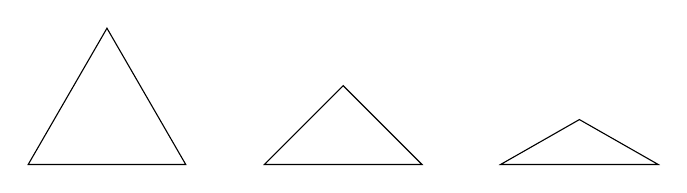
\begin{tikzpicture}
        \draw (0,0) -- (2,0) -- (1,1.73) -- cycle;
        \draw (3,0) -- (5,0) -- (4, 1) -- cycle;
        \draw (6,0) -- (8,0) -- (7,0.57) -- cycle;
    \end{tikzpicture}
    \label{fig:trianglemajo}
    \caption{We have respectively \((\pi/3, \pi/3,\pi/3) \prec (\pi/2,\pi/4, \pi/4) \prec (2\pi/3,\pi/6,\pi/6)\)}
\end{figure}
Here are some basics properties of majorization.
\begin{proposition} Let \(x,y\in\R^n\), \(\prec\) defines a partial order on \(\R^n\). Moreover,
    \begin{itemize}
        \item If \(x\prec y\) and \(y\prec x\), then there exists a permutation \(\pi\) such that \(\pi\cdot x = y\).
        \item If \(x\prec y\), then for any permutations \(\pi,\pi'\) we have \(\pi\cdot x\prec \pi'\cdot y\).
        \item We have \(\lvert x\rvert u\prec x \prec \lvert x\rvert\delta\) where \(u\) is the uniform distribution and \(\delta\) is the Dirac distribution.
    \end{itemize}
\end{proposition}
Note that \(\prec\) is \textit{indeed} a partial order. There exists vectors \(x,y\) such that neither \(x\prec y\) nor \(y\prec x\).
\\
Before going further, I will present a more information theoretic approach of majorization.
\begin{definition} A matrix \(A\in\R_+^{n\times n}\) is said to be stochastic if \(u^TA = u^T\).
    Moreover, we say that \(A\) is doubly stochastic if \(u^TA = u^T\) and \(Au = u\).
\end{definition}
A stochastic matrix \(A\) can be considered in the finite case as a so-called \textit{transition matrix} of a Markov chain. 
These are considered as the most basic representation of \text{channels} in information theory.
\begin{tikzcd}
    \text{source} \arrow[r, "A"] & \text{destination}
\end{tikzcd}
\section{Generalized (?) majorization}
We consider \((\mathfrak{X},\mathcal{X})\)  be a measurable space.

We want to generalize the concept of doubly stochastic matrices. As a reminder, a doubly stochastic matrix is a matrix \(A\in\R^{n\times n}\) such that
\begin{align}
    u^TA &= u^T\\
    Au &= u.
\end{align}
The first condition is only defining \(A\) as a proper Markov kernel in the finite case.
The second condition must be interpreted as the fact that \(A\cdot \mathcal{U}\) where \(\mathcal{U}\) is the uniform distribution on \(\{1,...,n\}\).
Therefore, we can generalize the concept of doubly stochastic matrices as follows. 

For a given probability measure \(\mathcal{U}\) on \((\mathfrak{X},\mathcal{X})\), \(K\) is 
said to be doubly stochastic kernel if it is \(\mathcal{U}-\)invariant.

\begin{example} Let \(\mathfrak{X} = [a,b]\) and \(\mathcal{U} = \mathbf{1}_{[a,b]}\), then \(K\) is 
    a double stochastic kernel if and only if \(K\) verifies 
    \begin{equation}
        \mathcal{U}(A) = \int_A \mathcal{U}(dx) K(x,A) = \frac{1}{b-a} \int_a^b K(x,A)dx
    \end{equation}
    Hence 
    \begin{equation}
        \int_a^b K(x,A)dx = \mathrm{Vol}(A).
    \end{equation}
\end{example}

\begin{definition}
    We say that \(\mu\) is majorized by \(\nu\), denoted \(\mu\prec \nu\), if there exists a doubly stochastic kernel \(K\) such that
    \begin{equation}
        \mu = K\nu.
    \end{equation}
\end{definition}
\begin{proposition} \(\prec\) is partial order on the set of probability measures on \((\mathfrak{X},\mathcal{X})\).
\end{proposition}
\end{document}
